% !TeX encoding=unicode
% !TeX spellcheck = de-DE

\chapter{The considered process: Higgs production through gluon fusion}
\label{ch:gfusion}
The Englert-Brout-Higgs-Guralnik-Hagen-Kibble mechanism (commonly Higgs mechanism) explains the non-zero masses of the gauge bosons in the standard model.
It has been developed in the 1960s with important contributions coming from several people \cite{higgs1964a,higgs1964b,englert1964,guralnik1964,nambu1960,anderson1963}.
It invokes the process of spontaneous symmetry breaking and evades the Goldstone theorem.
In the development of the standard model, the Higgs mechanism played a key role and ever since the discovery of a Higgs boson in 2012 by ATLAS \cite{higgsdiscovery_atlas2012} and CMS \cite{higgsdiscovery_cms2012} at the LHC it has received wide approval.

In this thesis, the considered process is the production of a Higgs boson through gluon fusion.
Accurate theoretical predictions of the differential observables are crucial to the analysis of the properties of the discovered particle.
This chapter provides a description of the gluon fusion process and its features.
\Cref{sec:higgs_pt} addresses the distribution of the transverse momentum in particular.
%
\section{Gluon fusion at the LHC}
Although there are other possible production mechanisms in the Standard Model, gluon fusion is the main process at the LHC, with an expected cross section of $\approx \SI{50}{\pico\barn}$ at a center of mass energy of $\sqrt{s} = \SI{14}{\tera\electronvolt}$ and a Higgs mass of $\SI{125}{\giga\electronvolt}$ \cite{higgshandbook1}.
It proceeds through a triangular loop of heavy quarks (mainly top quarks as the Higgs coupling scales with the quark mass) as is shown in \figref{fig:gluonfusion}.
%
\begin{figure}[]
	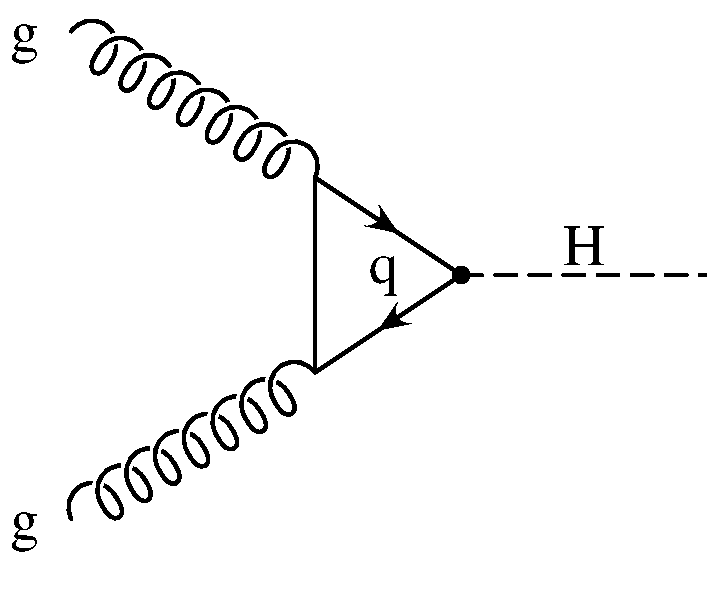
\includegraphics[width=0.5\textwidth]{images/gluonfusion.pdf}
	\caption{Higgs production through gluon fusion.}
	\label{fig:gluonfusion}
\end{figure}
%

In the narrow-width approximation, the leading order cross section is given by \cite{gluonfusioncrosssection}
%
\begin{equation}
	\sigma_\text{LO}(pp \rightarrow H) = \sigma_0^H \tau_H \od{\lumi^{gg}}{\tau_H} \, ,
\end{equation}
%
where $\tau_H = M_H^2/s$ is the Drell-Yan variable and $\dif \lumi^{gg} / \dif \tau_H$ is the gluon luminosity.
The partonic cross section $\sigma_0^H$ can be written as
\begin{equation}
	\sigma_0^H = \frac{G_F \alpha_s^2(\mu_R^2)}{288 \sqrt{2} \pi} \abs{ \sum_q \frac{3}{2 \tau_q} \left[ 1 + \left( 1 - \frac{1}{\tau_q} \right) f(\tau_q) \right] }^2  \, ,
\end{equation}
%
with the form factor
%
\begin{equation}
	f(\tau_q) = 
	\begin{cases}
		\arcsin^2 \left( \sqrt{\tau_q} \right) ,																& \tau_q < 1, \\
		- \frac{1}{4} \left[ \ln \frac{1 + \sqrt{1-\tau_q^{-1}}}{1 - \sqrt{1-\tau_q^{-1}}} -i \pi \right]^2 ,	& \tau_q > 1,
	\end{cases}
\end{equation}
%
where $G_F$ denotes the Fermi coupling constant and $\tau_q = m_H^2/4m_q^2$.
The gluon luminosity takes the form
%
\begin{equation}
	\od{\lumi^{gg}}{\tau_H} = \int_0^1 \dif x_1 \dif x_2 \gluonpdf(x_1,\mu_F^2) \gluonpdf(x_2,\mu_F^2) \delta(x_1 x_2 - \tau_q) \,
\end{equation}
%
with $\gluonpdf(x,\mu_F^2)$ denoting the gluon PDF.

The QCD corrections are composed of virtual corrections to the vertices and propagators, real gluon radiation in the initial state and the contributions of the subprocesses $gq \rightarrow Hq$ and $q \bar q \rightarrow Hg$.
Exemplary diagrams for the corrections are shown in \figref{fig:ggh_corrections}.
The full NLO cross section has been calculated in \cite{gfusionnlo1,gfusionnlo2,gfusionnlo3}.
They increase the cross section by a factor of \num{1.5} to \num{1.7}.
%
\begin{figure}
\centering
\begin{subfigure}[]{0.3\textwidth}
	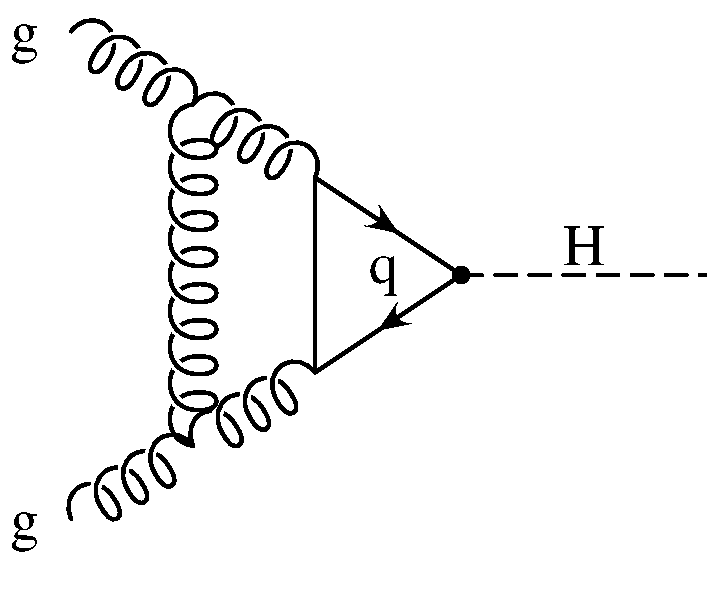
\includegraphics[width=\textwidth]{images/gluonfusion_virtual1.pdf}
	\caption{}
\end{subfigure}
~
\begin{subfigure}[]{0.3\textwidth}
	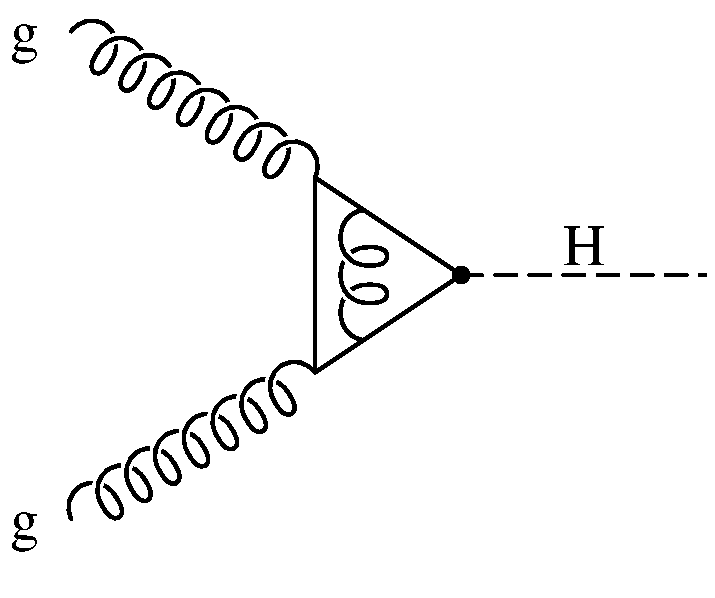
\includegraphics[width=\textwidth]{images/gluonfusion_virtual2.pdf}
	\caption{}
\end{subfigure}
~
\begin{subfigure}[]{0.3\textwidth}
	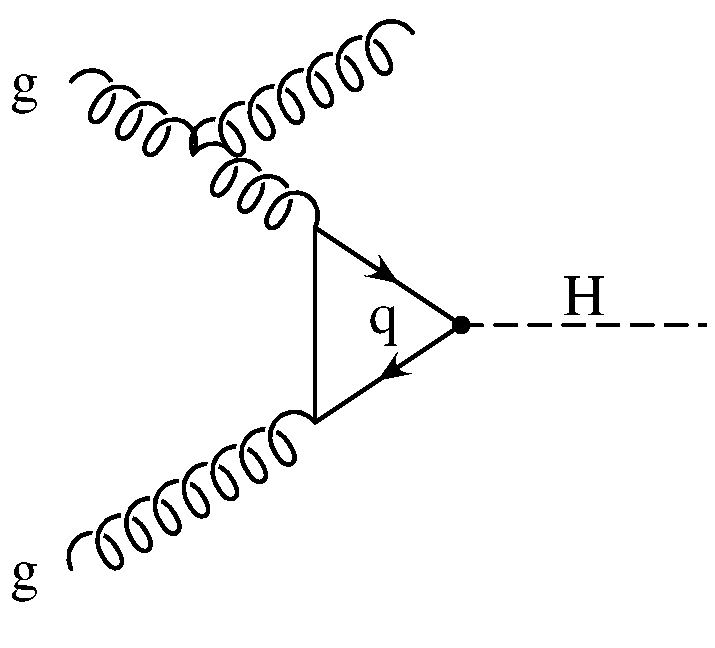
\includegraphics[width=\textwidth]{images/gluonfusion_real1.pdf}
	\caption{}
\end{subfigure}

\begin{subfigure}[]{0.3\textwidth}
	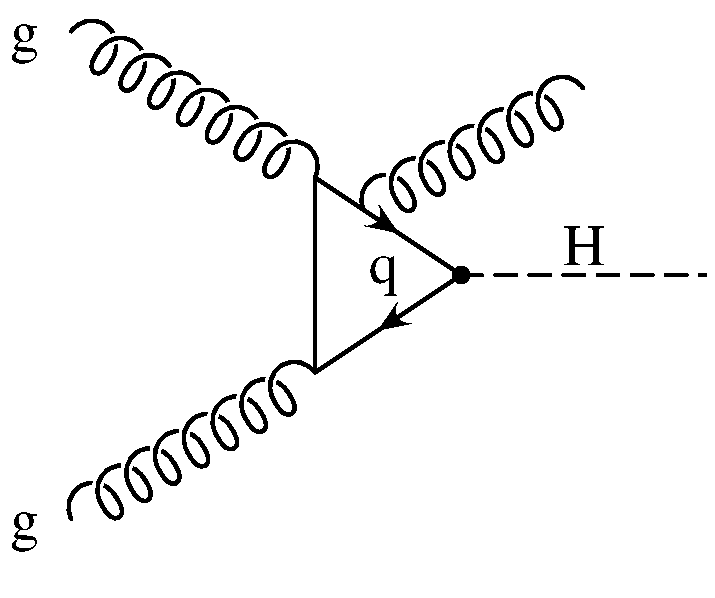
\includegraphics[width=\textwidth]{images/gluonfusion_real2.pdf}
	\caption{}
\end{subfigure}
~
\begin{subfigure}[]{0.3\textwidth}
	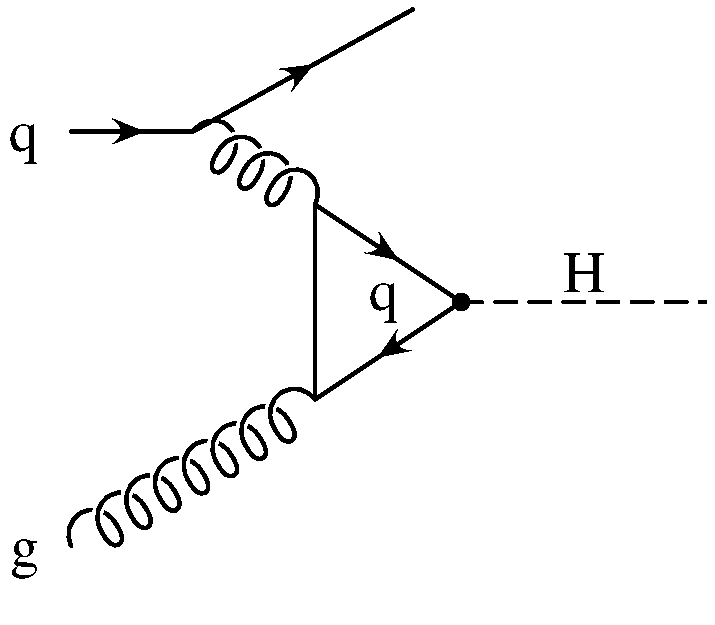
\includegraphics[width=\textwidth]{images/gq_hq.pdf}
	\caption{}
\end{subfigure}
~
\begin{subfigure}[]{0.3\textwidth}
	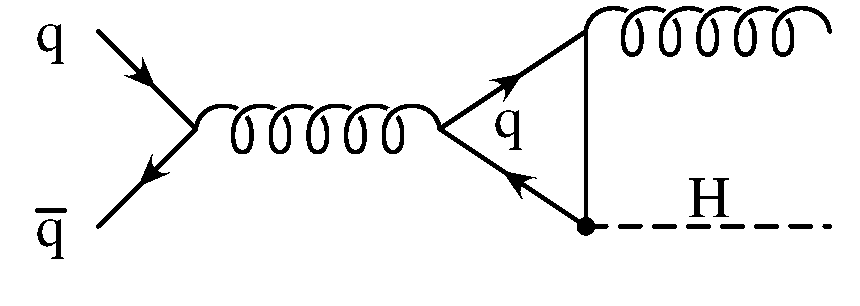
\includegraphics[width=\textwidth]{images/qq_hg.pdf}
	\caption{}
\end{subfigure}
\caption{Example diagrams illustrating the QCD corrections to the process $pp \rightarrow H$:
		(a), (b) virtual corrections; (c), (d) real emission of a gluon; (e) $gq \rightarrow Hq$; (f) $q \bar q \rightarrow Hg$.}
\label{fig:ggh_corrections}
\end{figure}
%

In the limit where the top quark has infinite mass, $m_t \rightarrow \infty$, the form factor takes the value $\frac{4}{3}$.
This allows for an analytical expression of the corrections \cite{gfusionnlo2}.
This approximation can be considered as an extension of the Standard Model, where the Higgs boson couples directly to gluons, known as effective Higgs coupling (cf. \cref{fig:heft}).
The effective Lagrangian for Higgs gluon interaction can be written as \cite{gfusionnnlo2}
%
\begin{equation}
	\Lagr_\text{eff}^{ggH} = - \frac{1}{4v} C_1 G_{\mu \nu}^a {G^a}^{\mu \nu} H \, ,
\end{equation}
%
where $v$ is the Higgs vacuum expectation value, $G^a_{\mu \nu}$ is the gluon field strength tensor and $H$ is the Higgs field.
The coefficient $C_1$, in the \msbar{} scheme, is given by
%
\begin{align}
	C_1 = \frac{-1}{3 \pi} &\left\{1 + \frac{11 \alpha_s}{4 \pi} + \left( \frac{\alpha_s}{\pi} \right)^2 \left[ \frac{2777}{288} + \frac{19}{16} \log\left( \frac{\mu^2}{m_t^2} \right)
	\vphantom{n_f \left( -\frac{67}{96} + \frac{1}{3} \log\left( \frac{\mu^2}{m_t^2} \right) \right)} \right. \right. \nonumber \\
	%	
		&\qquad \left. \left. \vphantom{\frac{2777}{288} + \frac{19}{16} \log\left( \frac{\mu^2}{m_t^2} \right)}
		+ n_f \left( -\frac{67}{96} + \frac{1}{3} \log\left( \frac{\mu^2}{m_t^2} \right) \right) \right] + \order{\alpha_s^3} \right\} \, ,
\end{align}
%
where the number of active flavors should be set to $n_f = 5$.
According to \cite{gfusionnnlo2}, at LO this approximation is accurate within \SI{5}{\percent} for $m_H \approx \SI{150}{\giga\electronvolt}$ (which is close to the measured value $m_H \approx \SI{126}{\giga\electronvolt}$) and improves at NLO.
All calculations in this thesis are based on effective Higgs coupling.
%
\begin{figure}[]
	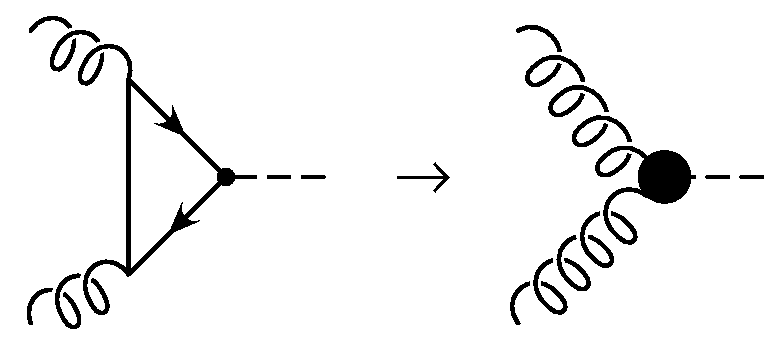
\includegraphics[width=0.5\textwidth]{images/heft.pdf}
	\caption{Effective Higgs coupling.}
	\label{fig:heft}
\end{figure}
%

Besides the basic process, the fully differential NLO cross sections are available for $H + 1$ jet \cite{gghj_nlo_fullydiff_1,gghj_nlo_fullydiff_2}, $H + 2$ jets \cite{gghjj_nlo_fullydiff_1,gghjj_nlo_fullydiff_2} and $H + 3$ jets \cite{gghjjj_nlo_fullydiff}.
A fully differential NNLO calculation exists for $H + 0$ jets production \cite{ggh_nnlo_fullydiff_1,ggh_nnlo_fullydiff_2} and substantial progress has been achieved towards an NNLO calculation of the $H + 1$ jet cross section \cite{gghj_nnlo_progress}.
%
\section{Leptonic Higgs decay}
In an experiment, one would never observe the Higgs boson directly but rather reconstruct it from the measured properties of its decay products.
We want to model this situation by simulating the Higgs boson decay.
There are several possible decay channels.
One has to keep in mind that the Higgs coupling is proportional to the particle masses, so that it will decay into the heaviest possible particles.
Assuming a Higgs mass of $m_H = \SI{126}{\giga\electronvolt}$, the most relevant decay products are $q \bar q$ (where q denotes a bottom or charm quark), $WW$, $ZZ$, $Z \gamma$, $\gamma \gamma$, $gg$ and $\tau^+ \tau^-$ \cite{higgshandbook2}.
The decay into photons or gluons is only possible through intermediate loops.
The studies leading to the discovery of the Higgs boson at the LHC relied primarily on the decay modes $H \rightarrow \gamma \gamma$, $H \rightarrow ZZ$ and $H \rightarrow WW$.

For the purpose of this thesis, the decay $H \rightarrow \tau^+ \tau^-$ is considered, which has a branching ratio of approximately \SI{6}{\percent} \cite{higgshandbook3}.
The Feynman diagram is shown in \cref{fig:h_tautau}.
It would be possible to simulate the other decay channels as well, however, this would only complicate the analysis unnecessarily.
The leptonic decay is the easiest one and closely resembles the Drell-Yan process.
There have been searches for $H \rightarrow \tau \tau$ events in the LHC data and both ATLAS \cite{htau_atlas} and CMS \cite{htau_cms} have published evidence for this type of decay.
It also allows for the observation of additional jets that are produced in the initial state and are separated from the Higgs decay products.
The further decay of the tau leptons, which would naturally occur in the experiment, will not be considered here.
%
\begin{figure}[]
	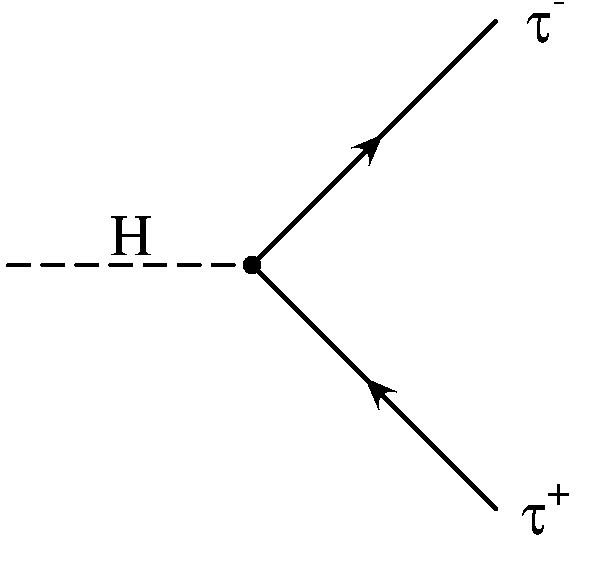
\includegraphics[width=0.3\textwidth]{images/h_tautau.pdf}
	\caption{Higgs decay into two $\tau$ leptons.}
	\label{fig:h_tautau}
\end{figure}
%
\section{The transverse momentum of the Higgs boson}
\label{sec:higgs_pt}
The transverse momentum distribution of the Higgs boson is one of the most interesting observables in Higgs production.
It provides a powerful test of the standard model once the statistics of the experimental results become suitable.
In the following, we will briefly study the distribution in the gluon fusion process, where the Higgs boson is produced along with different numbers of jets.
In particular, we take a look at how the quality of the prediction is influenced by parton showers.
Four separate runs have been performed: One run each for zero, one and two jets at fixed order NLO and one \mcatnlo{} run merging up to two jets in the core process.
The \rivet{} analysis system has been used to extract the transverse momentum of the Higgs boson from the events.
In the multijet merged run, the cases of at least zero, one or two jets have been distinguished and sorted into different histograms.
Thus, we obtain inclusive observables that are comparable to the fixed order results.
\sherpa{} has been used for all calculations and the \mcfm{} library \cite{mcfm_hjj} has been interfaced for the 2-jet process.
For the fixed order calculations, both the renormalization and the factorization scale have been set to the transverse mass of the Higgs boson.
Final state jets have been extracted by the \fastjet{} library \cite{fastjet_manual} using the anti-$k_t$ algorithm \cite{anti_kt} with a radius parameter $R=0.4$ and a $p_\perp$-cut of $p_\perp > \SI{20}{\giga\electronvolt}$.
All the resulting histograms have been normalized to \num{1}, so that the comparison is not affected by differences in the scale definitions between the fixed order and the merged runs.
As we want to do a qualitative study rather than a quantitative one, this is no big restriction.
For the same reason no uncertainties are shown in the plots.
More detailed studies can be found in the relevant literature, cf. for example \cite{symmetrybreaking1,symmetrybreaking2} or \cite{higgshandbook1,higgshandbook2,higgshandbook3}.

\Cref{fig:h_hpt_nominal} compares the fixed order NLO and the merged \mcatnlo{} results in the case of no jets.
At NLO the transverse momentum of the Higgs boson arises solely from real gluon emissions as the LO process does not have any transverse parts.
The splitting leading to the real emissions is divergent in the soft and collinear limits which correspond to low transverse momenta.
Therefore, in \cref{fig:h_hpt_nominal}, we see that the cross section diverges towards low $p_\perp$.
The multijet result behaves completely different in the low $p_\perp$ region and shows no divergence.
In this case, the cross section is dominated by parton showers which include higher orders and are not divergent.
Compared to the fixed order calculation, the cross section is much smaller in the low $p_\perp$ region.
As opposed to this, the cross section is amplified for $p_\perp \gtrsim \SI{20}{\giga\electronvolt}$.
The influence of the parton shower is negligible in this region.
Instead the additional contributions come from the higher jet multiplicities that have been merged into the calculation.
At high $p_\perp$, both results approach each other.
%
\begin{figure}
	\centering
	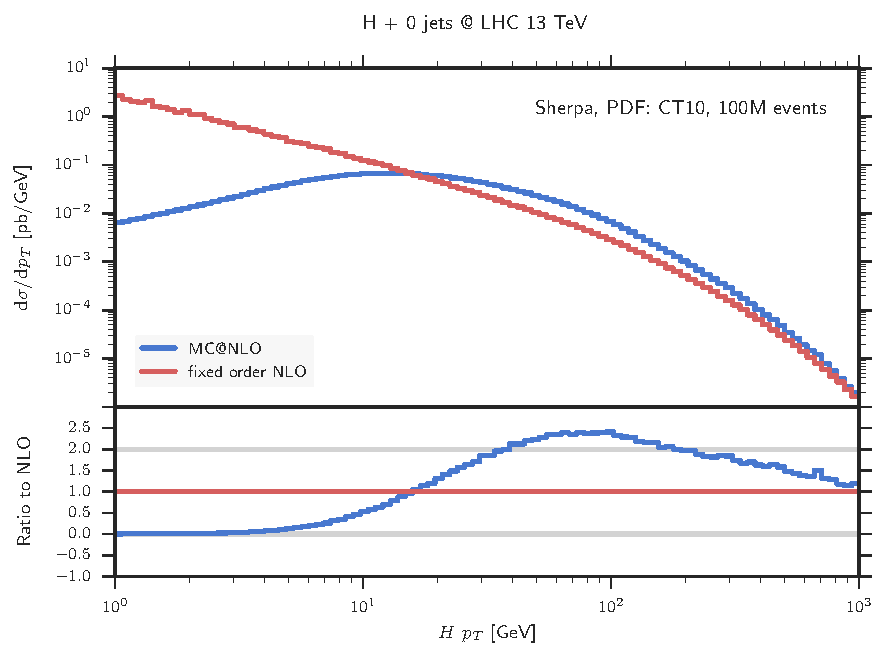
\includegraphics[width=0.8\textwidth]{images/h_hpt_nominal.pdf}
	\caption{Comparison of the Higgs transverse momentum distribution between an inclusive fixed order NLO calculation and a multijet merged parton shower matched \mcatnlo{} calculation with up to 2 jets.
	Note how the \mcatnlo{} result does not diverge in the low $p_\perp$ limit.}
	\label{fig:h_hpt_nominal}
\end{figure}
%

The results containing one or more jets are compared in \cref{fig:hj_hpt_nominal}.
Due to the jet cut, Higgs $p_\perp$ below \SI{20}{\giga\electronvolt} are very unlikely and present no meaningful observable, so we do not consider that case.
At $p_\perp = \SI{20}{\giga\electronvolt}$, when the Higgs boson recoils against the jet, the cross section diverges at NLO.
Similar to the previous situation, the parton shower fixes the divergence and produces a smooth distribution.
At high $p_\perp$ the merged run gives a higher cross section, this time the additional contributions stem from the 2-jet process.
%
\begin{figure}
	\centering
	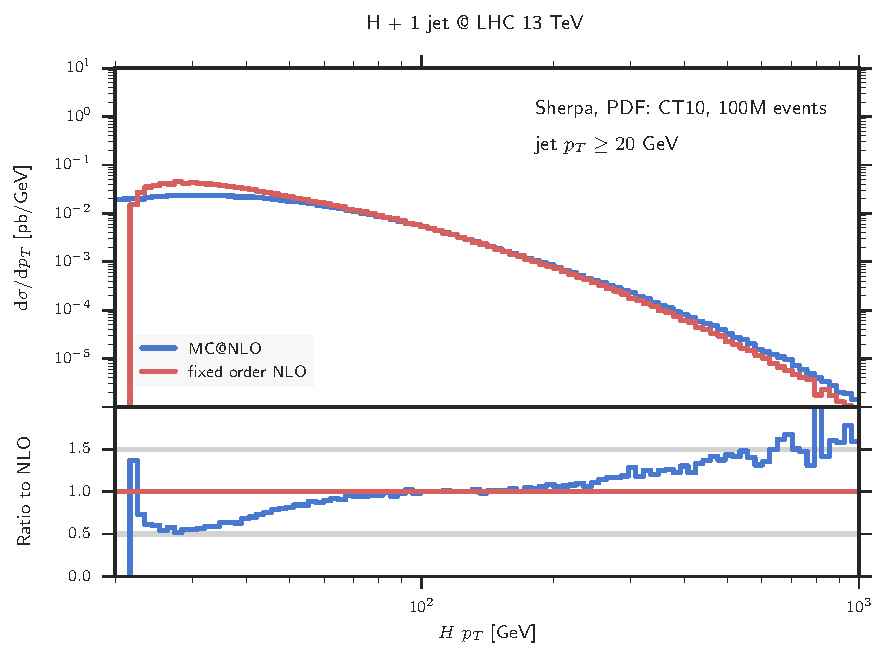
\includegraphics[width=0.8\textwidth]{images/hj_hpt_nominal.pdf}
	\caption{As in \cref{fig:h_hpt_nominal} with at least one anti-$k_t$ jet with $p_\perp \geq \SI{20}{\giga\electronvolt}$.}
	\label{fig:hj_hpt_nominal}
\end{figure}
%

With two additional jets, the fixed order and the showered result become very similar, cf. \cref{fig:hjj_hpt_nominal}.
The core process now is the same in both cases.
Higher multiplicities in the \mcatnlo{} result are generated only by the parton shower.
The influence of the shower, though, is negligible.
%
\begin{figure}
	\centering
	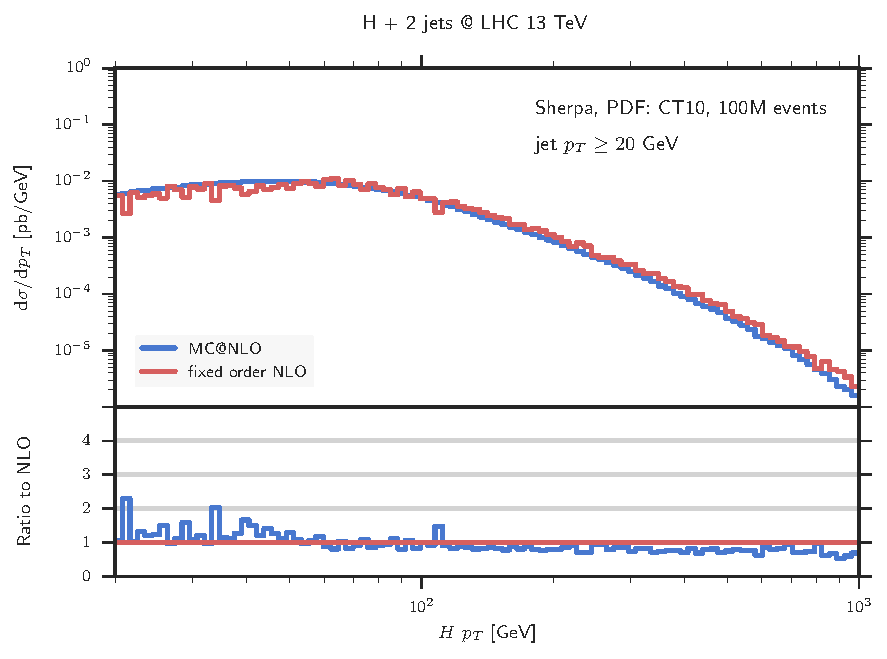
\includegraphics[width=0.8\textwidth]{images/hjj_hpt_nominal.pdf}
	\caption{As in \cref{fig:hj_hpt_nominal} with at least 2 jets.}
	\label{fig:hjj_hpt_nominal}
\end{figure}
%
